\section{Calibration System}
\label{sec:dp-pds-calibration}

\subsection{Goals of The Calibration System}

A photon calibration system is required in the DP module to calibrate the \dwords{pmt} installed in the \dword{lar} volume. The goal is to determine the \dword{pmt} gain and to monitor the stability of the \dword{pmt} response. One of the main goals of the \dword{pds} is to provide trigger for non-beam physics. The trigger is based on the amplitude of \dword{pmt}-signals. The amplitudes of the \dword{pmt}-signals are summed for groups of certain \dwords{pmt} and/or for all \dwords{pmt} and then, these input signals are discriminated according to the trigger logic. An equalized \dword{pmt} response allows to use the same threshold definition for all \dword{pmt} groups, simplifying the determination of the trigger efficiency. In addition to measuring the \dword{pmt} gain, the calibration system is also designed to monitor the stability of the \dword{pmt} response and its quantum efficiency. As concluded from the operation of a previous \num{3}$\times$\num{1}$\times$\num{1}\,m$^3$ \dword{lar} \dword{tpc} detector~\cite{Aimard:2018yxp} and the \dword{pmt} characterization at cryogenic temperature~\cite{Belver:2018erf}, a light calibration system is strongly recommended during the experiment data taking period.

%%%%%%%%%%%%%%%%%%%%%%%%%%%%%%%%%%%%%%%%%%%%%%%%%%%%%%%%%%%%%%%%%%%%

\subsection{Calibration System Design}

An \dword{led}-driven fiber calibration system~\cite{Cuesta:2017nrs,Conrad:2015xta,Caccianiga:2003fm,ADAMSON2002325} is designed so that a configurable amount of light reaches each \dword{pmt}. The calibration light is provided by a blue \dword{led} of \SI{465}{\nm} using a Kapustinsky~\cite{KAPUSTINSKY1985612} circuit as \dword{led} driver and transmitted by a fiber system ending with an optical fiber installed at each \dword{pmt} (see Fig.~\ref{dppd-6-LCS}). There are 20 groups of 6 \dwords{led} placed in a hexagonal geometry and a reference sensor to check the \dword{led} performance in the center of each group. The direct light goes to the fiber, and the stray light to the \dword{sipm} used as reference sensor. Each \dword{led} is connected to an external fiber going to one feedthrough. Then, fibers are connected inside the cryostat and each one of these fibers is attached to a 1-to-7 fiber bundle, so that one fiber is finally installed pointing at each \dword{pmt}. The \dwords{pmt} are oriented with the first dynode perpendicular to the Earth magnetic field and the fiber parallel to the first dynode to have a similar gain to the one obtained with diffuse light. The components placed outside the cryostat at room temperature form the \textit{external system} and the ones installed inside it at cryogenic temperature the \textit{inner system}. 

%############################################
%\begin{figure}[ht]
%\bigskip
%\centering
% \includegraphics[height=0.6\textwidth]{graphics/LCSdiagram_DUNE.pdf}
%\caption{Sketch of the \dword{dune} \dword{fd} \dfirst{pds} light calibration system. The external system at room temperature is shown in blue and the inner system at cryogenic temperature in black.}
%\label{dppd-6-LCS}
%\end{figure}

\begin{dunefigure}[Sketch of the \dword{dune} \dword{fd} \dfirst{pds} light calibration system.]{dppd-6-LCS}
{Sketch of the \dword{dune} \dword{fd} \dfirst{pds} light calibration system. The external system at room temperature is shown in blue and the inner system at cryogenic temperature in black.}
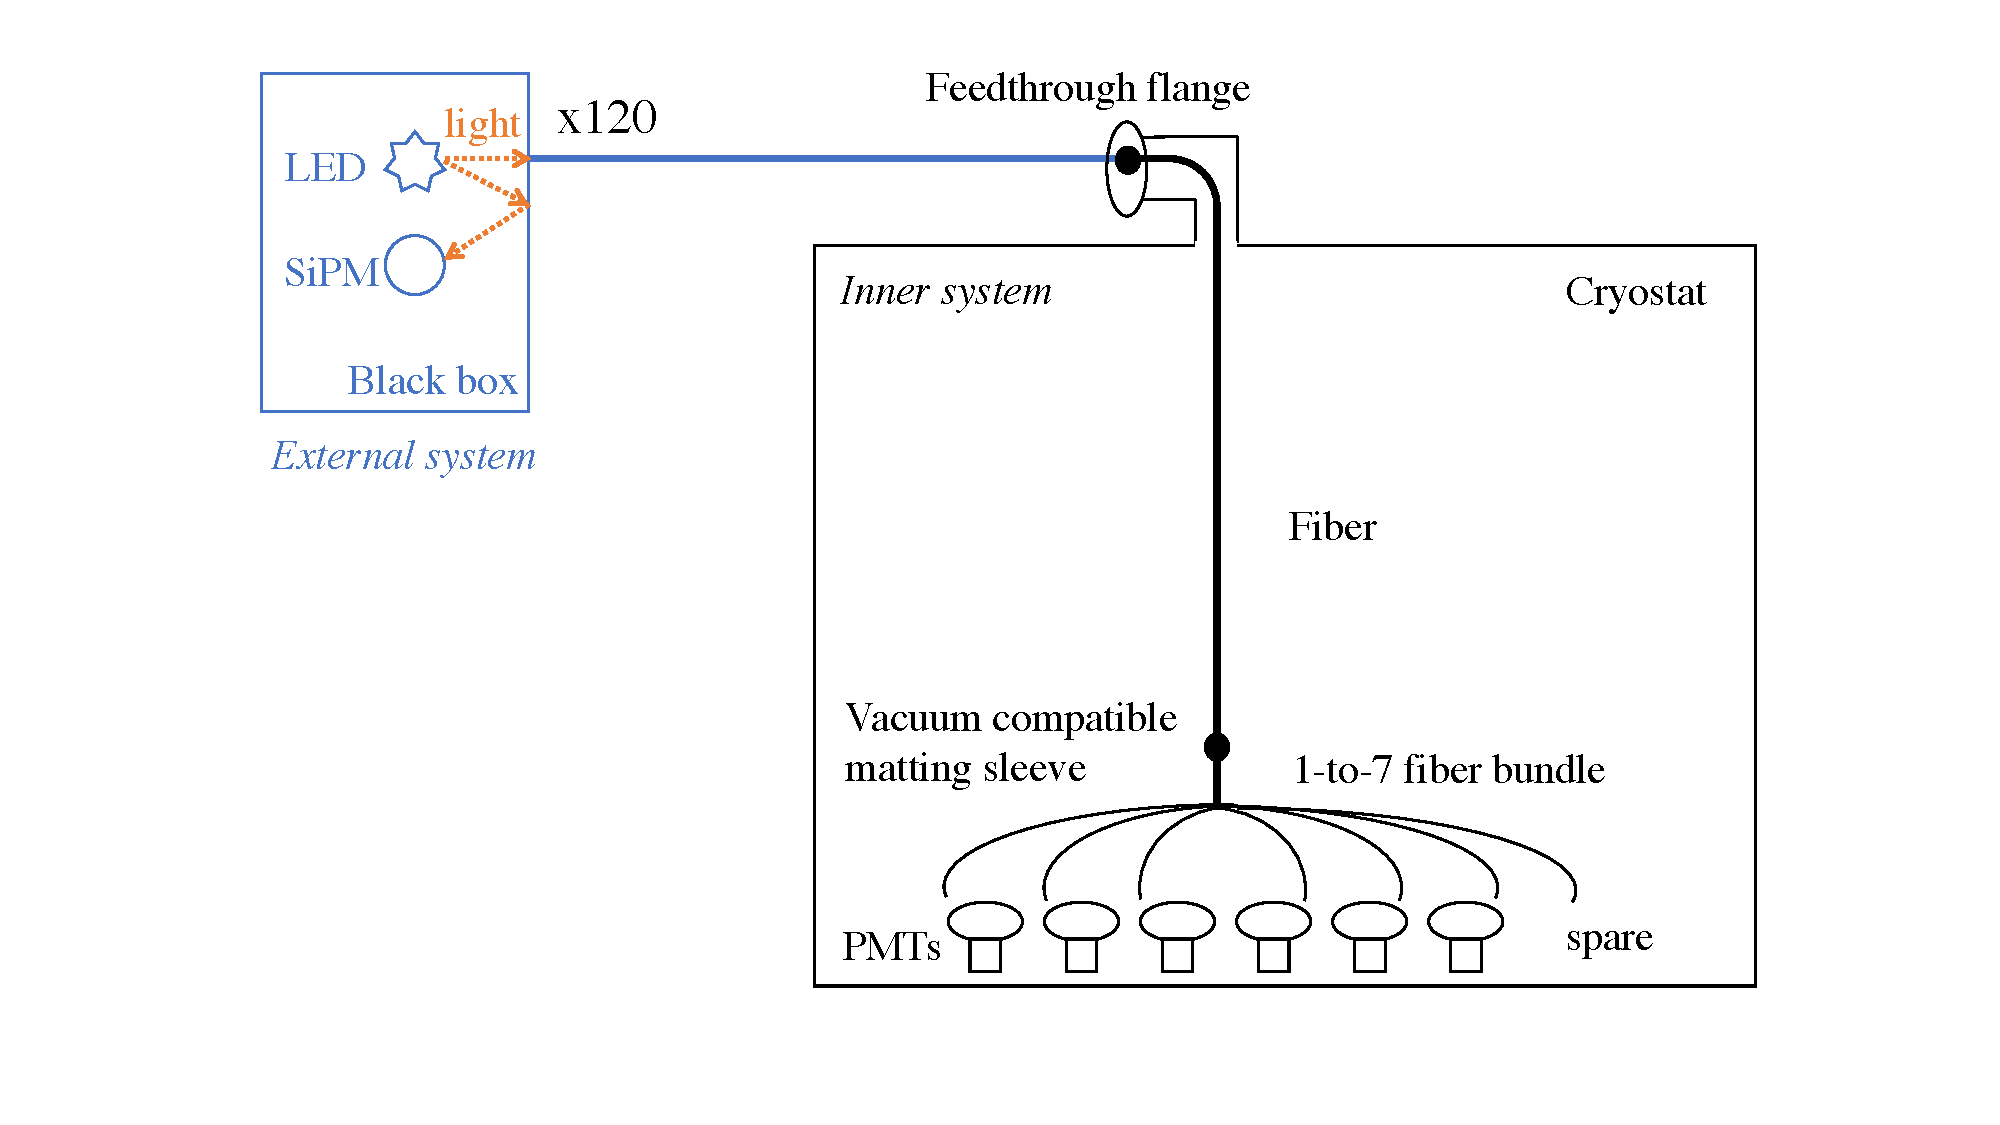
\includegraphics[width=0.7\textwidth]{dppd_LCSdiagram_DUNE}
\end{dunefigure}

%############################################

%%External system
The design of the external components is driven by the aim to have a cost-effective system. An additional requirement is that a reference light sensor monitors the amount of the injected light. The light is injected in form of several \si{\ns} long pulses provided by a Kapustinsky circuit. The setup consists of a commercial black box in which a light guide structure is mounted to guide the light. There are \num{20} structures, and each of them has six arms and a central part, as shown in Fig.~\ref{fig_source}. On each of the six arms, an electronics board containing a Kapustinsky circuit is mounted. The \dword{led}, NSPB300B from Nichia Corp.\footnote{www.nichia.com}, with a peak wavelength of \SI{465}{nm} is placed  on the PCB in front of an optical SMA to SMA feedthrough. On the other side of each feedthrough an optical fiber, FG105LCA-CUSTOM-MUC from Thorlabs\footnote{www.thorlabs.com}, is connected. It transports the light to one of the \num{120} feedthroughs in the instrumentation flange on top of the cryostat. While a large fraction of the LED light is emitted in the forward direction, a small fraction, the stray light, is emitted under a large angle and reaches by reflection to the central region of the light guide structure where it is detected by a \dword{sipm}, MicroFJ-30035-TSV-TA from SensL\footnote{www.sensl.com}.


%############################################
%\begin{figure}[h!]
%\centering
%\includegraphics[width=0.25\textwidth]{graphics/LightGuide.jpg}\label{fig:lightguide}
%\includegraphics[width=0.55\textwidth]{graphics/Stray.png}\label{fig:stray}
%\caption{(Left) Picture of the light guide structure during the development phase. The six arms are visible, and on one of them a prototype \dword{led} driver is mounted. (Right) Schematics of the light way from the \dword{led} to the reference sensor.}
%\label{fig_source}
%\end{figure}

\begin{dunefigure}[Picture of the light guide structure during the development phase and the schematics of the light way from the \dword{led} to the reference sensor.]{fig_source}
{(Left) Picture of the light guide structure during the development phase. The six arms are visible, and on one of them a prototype \dword{led} driver is mounted. (Right) Schematics of the light way from the \dword{led} to the reference sensor.}
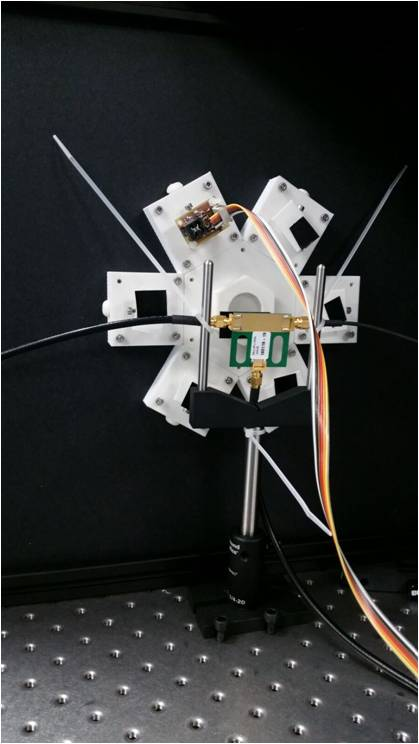
\includegraphics[width=0.25\textwidth]{dppd_LightGuide.jpg}
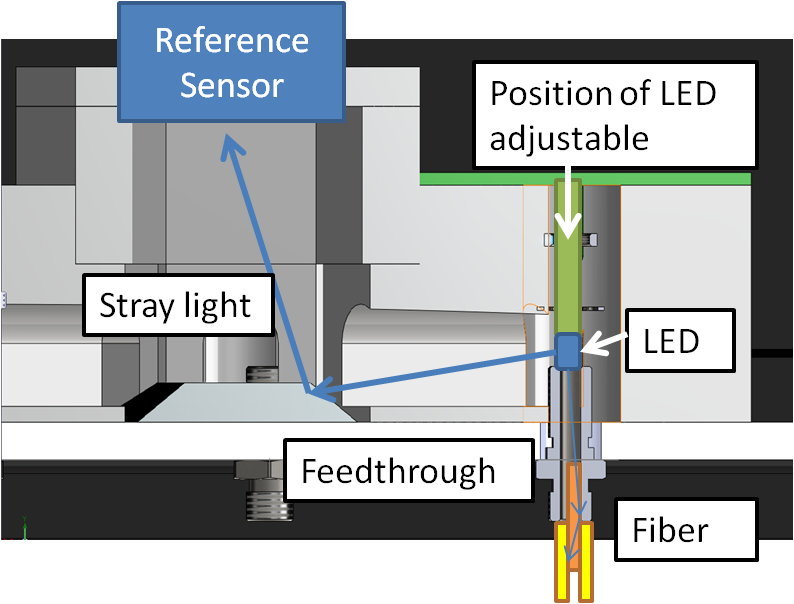
\includegraphics[width=0.6\textwidth]{dppd_Stray.png}
\end{dunefigure}




%############################################

%%Inner system
The inner system is designed to minimize the light losses at cryogenic temperature. The external fibers are connected to 120 female optical feedthroughs from Allectra\footnote{www.allectra.com} installed at \num{20} flanges. Inside the cryostat, a single long fiber, FT800UMT from Thorlabs, goes down from each optical feedthrough routed along the walls of the cryostat to its bottom where a \num{1}-to-\num{7} fiber bundle, composed by FT200UMT fibers from Thorlabs, is connected to each long fiber. A total of \num{720} of these fibers are guided to the \dwords{pmt} at the bottom of the detector. The end of the fiber is fixed at the \dword{pmt} support structure pointing the photocathode. The fibers and bundles are \num{0.39}\,NA TECS$^\text{TM}$ hard-clad, multimode, step-index fibers with high OH to increase the light transmission at low wavelengths. In order to optimize the light transmission of the fiber-bundle connection, the inner fibers have a diameter of \SI{800}{\um}, big enough to distribute uniformly the light at the bundle entrance, total diameter \SI{700}{\um}. From the mechanical point of view, the described approach of bundles attached to fibers is safer than connecting directly the bundles to the feedthroughs. To have good homogeneity of the light at the fiber-bundle connections, SMA connectors are chosen. Vacuum compatible SMA to SMA mating sleeves are required to avoid \dword{lar} to freeze inside the connector which would reduce the light transmission.

\fixme{Alternatives to illuminate many \dwords{pmt} at once with fibers on top of field cage being investigated for \dword{pddp}. If we end up installing such an alternative design in \dword{pddp}, we should adapt text here.}

%Alternatives to this design will be pursued with R\&D measurements in order to make  it  more  effective,  reduce  the  cost and  mitigate  issues  related  to  the  scaling. These alternatives include reducing the amount of fibers, studying other options for the reference sensor, and increasing the input light if necessary. To reduce the number of fibers, light diffusers can be used, so that one fiber can illuminate at least 4 PMTs. For instance, a diffuser could be placed at the ground grid.

%%Validation measurements
%In order to validate the design, the most important result comes from the ProtoDUNE-DP performance. In any case, since the fibers to be used in DUNE FD will be longer, dedicated calculations and measurements to confirm that sufficient light reaches the PMTs will be performed. Also, alternative designs, will be validated in different laboratories.  The possibility of using a diffuser can be tested in a vessel. The light source will also be validated by studying the different options in the lab. All these measurements will be performed at room temperature and in liquid nitrogen to test the behavior at cryogenic temperatures. Once the design is fixed, basic characterization measurements will be performed on the fibers upon receiving them from the manufacturer. Those measurements will consist of providing light with a known source and measuring the output with a power meter. Measurements at cryogenic temperatures may not be needed at this point.

%Finally, during the photon calibration system installation, each fiber and source will be re-tested to check that the expected light is arriving to each PMT using a photodiode. A dedicated procedure will be designed with this purpose, similar to the one used in ProtoDUNE-DP.
